\documentclass[a4paper, 11pt]{article}
\usepackage[pdftex]{graphicx}
\begin{document}
\tableofcontents
\section{Correctness}
\subsection{Transactions}
We have a set of Threads $T$ each representing a transaction.The code for a 
Transaction is like below:

\hspace{12mm}	Thread.doIt(new Callable)()\{

\hspace{12mm}		// code for transaction

\hspace{12mm}	\}

This is adopted from dstm and can and may be changed. Within this block which represents a member of set $T$. The functions beginTransction and endTransaction are implicitly called by the system without the intervention of the programmer.However, the programmer can read and write from TransactionalFile Objects within the blocks of a member of $T$. To provide consisteny the read and write from ordinary Java object files should be prohibited, otherwise the semantics of transactions would not be preserved. Hence, the sequence of operations provided to the programmer within a member of $T$ is the set \{TransactionalFile.Read(), TransactionalFile.Write()i, TransactionalFile.Seek()\}. However, always a beginTransaction() and commitTransaction() (if the transaction does not abort prior to this point) are performed too. \\ 

A Transaction consists of a sequence of operations. Thus, a transaction can be represented as the \{$op_1$, $op_2$, ..., $op_n$\}. The flow of program should be in a manner that we could have an arbitrary serial order of the members of $T$ (e.g. $T_5,T_6,T_1$,...) or any other order. The serial order should be in such a way that for any given two members of the set $T$, it looks all the operations of one occur before all the operation of the other. %In the first case we would say the $T_i$ precedes $T_j$ and in the seconds case $T_j$ preceds $T_i$ and $T_i$ can observe all the effects made by the operations in $T_j$. \\

\subsection{Defenitions}

textbf{Def 1-} \emph{Set of Primitive Operations}: Operations are taken from the set \{forcedreadoffset(filedescriptor), writeoffset(filedescriptor), readdata(inode, offset, length), writedata(inode, offset, length), commit\}. We denote read operations as readoffset and readdata and write operations as writeoffset and writedata.\\

\textbf{Def 2-} \emph{Operations Sharing Resources} 1- A forcedreadoffset operation and writeoffset operations are said to be sharing resources if they both operate on the same filedescriptor. 2- A readdata and writedata operations are said to be sharing resources if they both operate on the same inode AND the range of (offset, offset + length) within one overlaps with that of the other.\\ 

\textbf{Def 3-} A read operation can only see the writes made by write operations sharing reources.\\ 

\textbf{Def 4-} \emph{Commit Instant and Commit Operation}: A transaction commits when it invokes the "commit" operation. A transaction $T_i$ is said to "commit" at instant $t_i$, if and only if it reflects its "writes" made by write operations in the filesystem or equivalently makes it writes visible to the whole system for all members of $T$ accesing the data at instant $t_j$ such that $t_j > t_i$. After a transaction invokes commit operation, the transactin ends and no more operation by transaction is done. An operation $\in OP_{T_i}$ is said to commit if and only if $T_i$ commits. Commit instant are not splittable, hence it appears to other transactions that all writes are refleted in the file system together.\\ 

\textbf{Def 5-} \emph{Precedence Relationship}: If $OP_{executed} = \{op_0, op_1, ..., op_n\}$ represnts the operations executed so far(from all transactions running), and the indices represnt the order of operations executed so far in an ascending manner, we define $op_i \rightarrow op_j$ (precedes) if and only if $i<j$.\\ 

\textbf{Def 6-} \emph{Visbility of Writes}: Assume $T_i$ is an uncommitted transaction and $T_{commited}$ indicates the set of commited transaction (those which have invoked the "commit" operation). A read operation $b \in OP_{T_i}$ MAY ONLY see the writes(changes) made by preceding write operation $a$ that shares resources with $b$ AND also is subject to one of the following conditions:\\

\hspace{7mm} 1- $a \in OP_{T_j}$ ($j \neq i$) such that $T_j \in T_{commited}$ \\

\hspace{7mm} 2- $a \in OP_{T_i}$ and $a$ happens before $b$ in the natural order of the transaction. Formally, $a \rightarrow b$\\
 

\textbf{Corrolary 1-} \emph{No See in The Fututre}: If $ \exists op_i \in WRITEOP_{T_i}$ and $\exists op_j \in READOP{T_j}$ such that $i \neq j$ and $op_i \rightarrow op_j$ then if $op_j \rightarrow commit-operation_{T_i}$, writes made by $op_j$ are not seen by $op_i$.i\\

proof: Follows immediately from Def 5 and Def 6.\\

\textbf{Corrolary 2-} \emph{Read Must See Most Recent Comitted Write}: If $a \in OP{T_i}$ reads the resource $r_i$ at $t_i$. In case $a$ has multiple writer precedessors sharing $r_i$ (denoted as $OP_{precedessors-for-r_i}$), then if all of them are from sets other than $OP_{T_i}$, $a$ sees the writes made by $op_{T_j} \in OP_{precedessors-for-r_i}$ such that $T_j$ has the greatest "commit instant" less than $t_i$ between all transaction with such operations . Otherwise, $a$ sees the most recent precedessor in $OP_{T_i}$. \\

axiom: Assume $a$ is accessing data at $t_i$, according to Def 6, only writes by those transactions that have already committed would be visble. Hence, $t_i$ is neccasarily gretaer than all members of \{$committime_{T_1}, ..., commitime_{T_{i-1}}$\},and hence the writes to $r_i$ made by these commited transaction, have accroding to Def 4 been already reflected in the file system. Since, $T_{i-1}$ has the greatest commit instant its changes have overriden that of previously commited transactions and thus, $a$ reading $r_i$ from file system sees these changes.\\

In case 2 that there are writer operations writng $r_i$ and preceding $a$ in $OP_{T_i}$, according to defenition of transaction, $r_i$ should be read from the writes made by write operations in $T_i$, and as the last of such write operation overrides the written data to $r_i$ by other operations, $a$ gets to see the most recent precedessor in $T_i$.\\   


\textbf{Def 7-} \emph{Precedence Relationship For Transactions:} $\forall$ $op_{T_i}$ $\in OP_{T_i}$ and $\forall op_{T_j}\in OP_{T_j}$ if and only if $op_{T_i} \rightarrow op_{T_j}$ then $T_i$ $\rightarrow T_j$ \hspace{8mm} (this defines precedes relationship for members of $T$) \\

\textbf{Def 8-} \emph{Correctness:} A sequence of transactions are said to be consistent if and only if a total ordeing of them according to precedence relationship can be established that demonstrates the same behavior as the execution of the program. Behavior for an operation means the data it has read or wants to write. Demonstrating the same behavior thus means all the read operations should still see the same data in the new sequence as they have seen in the actual sequence. However writs always writes the same value no matter what. Hence the behavior of a write operation is not alterable.\\

\textbf{Note 1:} Def 7 and Def 8 indicate that if operations can be commuted in a given sequnce of $OP_{executed} = \{op_{T_1}(0), op_{T_4}(0), ... op_{T_1}(n)\}$ such that a total ordering of transactions (e.g \{$OP_{T_1}, OP_{T_2}, ..., OP_{T_n}) $\} can be obtained then the execution is consistent and correct. The eligiblity to commute is subject to conforming to Corrolary 1 \& 2.\\

\textbf{Def 9-} \emph{Relocation Operations in A Sequence}: In a sequence of operations $OP = \{op_1, op_2, ...,op_n\}$, any operation can relocate its position in the sequence unless as a result of this change, the behavior of a read operation changes (it reads different data).\\

\textbf{Note 2:} \emph{No Commute for Operations Belonging to The Same Transaction}: If $op_i \in OP_{T_i}$ and $op_{i+1} \in OP_{T_i}$, we never commute $op_i$ and $op_{i+1}$, since even if this exchange does not change any operations behavior, there is still no point in doing this as the aim is to put all operations belonging to the same transaction together, the internal order among these is not any of our concern, and the precedence relationship among these as indicated by the execution should be maintained.\\ 

\textbf{Note 3:} \emph{Precedence Relationship Between Commit Operations Should Be Preserved}: As a rquirement we want to have the notion that transaction are executed in the serial order imposed by their commit operations. Hence, commit operations can not be commuted.\\

All the rules explained later are based on the assumptions made in Note 2 \& 3, hence these two types of commution are ruled out by default.\\



\subsection{Rules}

\textbf{Rule 1-} $\forall op_i \in  OP{T_i}$, $\forall op_j \in  OP{T_j}$, $\forall op_k \in  OP{T_k}$, if $op_i \rightarrow op_k$ and  $op_k \rightarrow op_j$, then $op_i \rightarrow op_j$ \\

proof: Follows from the defenition of $\rightarrow$ \\


\textbf{Rule 2-} If $T_i \rightarrow T_k$ and $T_k \rightarrow T_j$ then $T_i \rightarrow T_j$ \\

proof: Follws from Rule 1 and Def 7. \\ 

\textbf{Rule 3-} \emph{Exchnaging Position of Consecutive Operations}: Formally having the sequence of operations $OP = \{op_1,...,op_i,op_{i+1},...,op_n\}$, if $op_i \in OP_{T_n}$ and $op_{i+1} \in OP{T_m}$ such that $ n\neq m$, $op_i$ and $op_{i+1}$ can exchange positions if and only if none of the follwing conditions apply:\\

\hspace{8mm} 1- If $op_i = {commit}$ and $op_{i+1} = {read}$ and $op_{i+1}$ reads $r_k$, and $\not \exists op_k$ in $OP_{T_m}$ such that writes to $r_k$, and if there  $exists op_l \in OP_{T_n}$ such that writes the data $r_k$, then $op_i$ and $op_{i+1}$ can not exchange positions.\\ 

\hspace{8mm} 2- If $op_{i+1} = {commit}$ and $op_{i} = {read}$ and $op_{i}$ reads $r_k$ and $\not \exists op_k$ in $OP_{T_n}$ such that writes to $r_k$, and if there $exists op_l \in OP_{T_m}$ such that writes the data $r_k$, $op_i$ and $op_{i+1}$ can not exchange positions.\\ 


\textbf{Proof}: According to Def 9, none of the operatios in the sequence should change behavior as the result of this exchange, however in this argument only $op_i$ and $op_{i+1}$ may change behavior as those are the only operations that their postions in the sequence is changed. However, since behavior is only defined for read operations, one of these without losing generality lets say $op_i$ should be a read operation on agiven resource $r_k$.\\

Now changing the $(op_i, op_{i+1})$ to $(op_{i+1}, op_i)$ changes the behavior of $op_i$ if and only if $op_{i+1}$ writes $r_k$ at the file system (all the previous precedessors are still the same, only $op{i+1}$ has been added). This means by defenition the $op_{i+1}$ should be a commit operation. And, if $op_{i+1}$ is a commit operation for $T_m$, and there is at least one write operation in $T_m$ writing to $r_k$, then according to Corrolary $op_i$ should see the most recent results and hence if there is no precedessor for $op_i$ in $T_n$ itself that writes to $r_k$, then $op_i$ sees the changes made by the write operarion in $T_m$. These changes could not have been seen in the first case $(op_i, op_{i+1})$ due to Corrolary 1 (No See in The Future).\\ 


\textbf{Rule 4} -\emph{Relocating the Position of an Operation Within the Sequence}: Given a sequence of operations $OP = \{op_1, ..., op_i, op_{i+1}, ..., op_j, op_{j+1}, ..., op_n\}$, $op_j$ can be put into the standing $i<j$ within the sequence (resulting in $OP = \{op_1, ..., op_i,op_j,op_{i+1},..., op_{j+1},...,op_n\}$) if and only if $\forall op \in \{op_{i+1}, ..., op_{j-1}\}$, $op$ and $op_j$ belong to different transactions and the pair $(op_j, op)$ or $(op,op_j)$ is not a pair subject to one of the conditions in Rule 3. The same holds true for $i>j$.\\

proof: We use induction to prove if assumptions above hold true $op_j$ can be relocated to $i = j-n$. Assume the same $OP$ as before. If $n = 1$ then since according to assumption the pair $(op_j, op_{j-1})$ is not subject to the conditions in Rule 3, these two can be easily exchanged. Now, lets assume the $op_j$ can be relocated to $j-n-1$, now we prove it for $n$.  After relocation to $j-n-1$, $op_{i+1}$ immediately precedes $op_j$, as according to assumption and Rule 3 $op_j$ and $op_{i+1}$ can exchange positions. After this exchange, $op_j$ has been relocated by $n$ and to $i$ and $op_i$ now immediately precedes $op_j$.\\

Now we prove the other side of the argument, that if $op_j$ can be relocated in $i$, $\forall op \in \{op_{i+1}, ..., op{j-1}\}, (op_j, op)$ is not a pair subject to the condition in Rule 3. Lets assume there is $op$ in $T_i$ such that $(op, op_{j})$ is a $({read r_n}, {commit})$  and the commit invlolves making a write in $T_j$ to $r_n$ durable and a precedessor writer that writes to $r_n$ does not exists for $op$ in $OP_{T_i}$ , now if $op_j$ is relocated to position $i$, $op_j$ would precede $op$ and hence $op$ would see the writes by the operation in $T_j$ (defenition of commit Def 4 \& Corrolary  2) and hence the behavior of $op$ would change as it does not read the same data as before (the data read before could not have been the same thing due to Corrolary 1). If the pair of $(op, op_j)$ is $({commit}, {read r_n})$ the same reasoning would do.\\   

The whole argument can be used to prove the Rule for $i > j$ as well.\\

\textbf{Rule 5-}\emph{Operation in the Set of Execeuted Operations Belonging to Committed Transactions Should Be Able To Precede Those in The Transaction About to Commit}: $OP_{executed} = \{op_1,..., op_n\}$ represents the set of executed operations before instant $t_j$ and $T_{committed}$ represents the set of committed transactions committed successfully before $t_j$. If $T_j$ invokes ${commit}$ operation at instant $t_j$ - then $T_j$ commits at instant $t_j$ if and only if operations in $OP$ can be commuted in a way such that $\forall op_i \in OP_{T{committed}}$, $\forall op_j \in OP_{T_j}$, $op_i \rightarrow op_j$.\\


proof: If all those operations can be commuted tp precede those in $T_j$ we could have $OP_{executed} = \{op_1,...,OP{T_j}\}$. This by defenition of transaction means $T_j$ can commit (it is executed in its whole entierty).\\

Now we have to prove $T_j$ commits only if $\forall T_i \in T_{committed} T_i \rightarrow T_j$. Now we'll show that if all committed operations can not precede operation of $T_j$ the $T_j$ can not commit. $OP = \{op_{T_j}(1), ..., op{T_j}(m)\}$ represent the operations in $T_j$ excluding the ${commit}$ in the order they have occured in $OP_{executed}$. Assume \{$op_{T_j}(k),...op{T_j}(m)$\} can be relocated in $OP_{executed}$ in the standing \{n-(m-k), ...,n-1) but $op_{T_j}(k-1)$ can not. This means first of all $op_{T_j}(k-1)$ is a ${read}$ operation reading $r_n$(each transaction has only one ${commit}$ operation).\\

Furthermore, this implies there is a ${commit}$ operation by some transactione $T_i$ between $op{T_j}(k-1)$ and commit operation by $T_j$ and $ \exists op in OP{T_i}$ such that writes $r_n$ and $\not \exists op_i \in OP{T_j}$ such that $op_i \rightarrow op_{T_i}(k-1)$. On the other hand since there is a ${commit}$ by $T_i$ in the middle, the commit by $T_J$ can not be commuted in a way so $OP$ precedes it without any operation belonging to other transaction in the middle (two ${commits}$ can not commute). Hence we can not have a sequence where all operations belonging to $T_j$ are located next to each other, this contradicts the defenition of transaction, hence the transaction can not commit.  


%\subsection{TransactionalFile Opeartions}
%TransactioalFiles can be either created inside or outside $T$. The TransactionalFile object ensures transactional access no matter where it is created and accessed. Meaning the first time $T_i$ \emph {uses} $tf_j$ the flow of the program should look like no other piece of code (i.e Transactional and non-transactional) outside $T_i$ will \emph {modify} $tf_j$ before $OP(endtransaction)_{T_i}$. Otherwise, $T_i$ has to abort. \\


%A Transactionalfile can be shared among any subset of the members of $T$. If shared, the offset is shared between these too. 

%\section{Implications for the System}

%\subsection{General Implications}
%Now, if $T_i$ and $T_j$ do not either write the data the other one reads, according to Rule 2 and 3 both can commit. This means even if $T_i$ accesses $r_k$ before $T_j$ does, but $T_j$ commits before $T_i$, given that $T_j$ has not modified the data in use by $T_i$, $T_i$ could still commit. \\


%It should be noted that according to Rule 3 even if all but one of the transactions in the set of committed transaction precede $T_i$ which is about to commit, , still the transaction can not commit. Therefore it takes only one operation to make the transaction dependent (all the committed transaction should precede this transaction but can not since one of the operations in the committed transaction does not precede an operation in this transaction). Formally, if there is an operation $b \in OP_{T_j}$ and an operation $a \in OP_{T_i}$ such that $a$ does not precede $b$ then $T_i$ can not precede $T_j$. In the rules below $T_i$ is not commited yet and $T$ denotes the set of all commited or active transactions. \\

%Assumption : The reads within transaction do actually occur when they are encountered. However, no change to the file system is done before commit instant as said before (writes, changing the offset and etc.)\\


%Assumption: seek operation means after this operation is executed, the offset should be at the chosen value regardless of the actual value of the offset in the file system.\\

%Principle 0: An operation should not see any modifications other than those made by precedessors (either in the same transaction or others)\\

%proof: Obviously such modifications are not valid and are probably part of a faulty operation.\\


%Principle 1) \emph{Reads Should be Validated At Commit Instant}: If an operation $a$ that "reads" some data $r_n$ (reads the data at some $t < t_{commit-of-the-transaction}$(the commit instant)), it should be ensured that the data $r_n$ is still valid in the actual file system at $t_{commit-of-the-transaction}$ (commit instant) or $T_i$ has to abort.\\

%proof: If the data is not valid anymore it means the data $r_n$ has been written since $t_{i-1}$. This implies at least one operation $b$ has written the data since the use and $b$ does not precede $a$ and $a$ precedes $b$. $b$ is either an operation in the same transaction or a different one. According to Def 4, however if $b$ is in the same transaction, then $b$ can not have commited yet and hence the changes are not reflected in the filesystem so it is still valid at commit instant. Hence, $b$ belongs to a different transaction namely $T_j$. Since $T_j$ should have already commited, according to Rule 3 all operation in $OP_{T_j}$ should precede those in $OP_{T_i}$, however, we know there is at least an operation $b$ that does not precede $a$ (since $a$ has not seen the "writes" made to $r_n$ by $b$). Hence, $T_i$ can not commit.\\

%The same reasoning could be done for $T_i$ and $T_{i-1}$, $T_{i-1}$ the last commited transaction before $T_{i}$. Now according to rule 3, since $T_j$ succeds $T_i$ and $T_i$ succeds $T_{i-1}$, hence $T_j$ succeds $T_{i-1}$. Same reasoning is applied for all the members of $T_{commited}$. \\ 

%Principle 2: emph{If Reads Are Valid At Commit Instant, the Transaction Commits}: If by applying Principle 1 for $T_i$ it is ensured that $\forall r_i \in R{T_i}$ (all data read by $T_i$) is still valid at commit instant, then $\forall T_j \in T_{committed} T_j \rightarrow T_j$ and hence according to Rule 4 $T_i$ commits.\\

%proof: If all data read is still valid at commit instant, means all operation in the set of operations belonging to committed transactions, precede those in $T_i$ (since no writes have been seen), and consequently all those transactions precede $T_i$.\\ 

%Principle 2) 1-A seek operation in $OP_{T_i}$ does not make $T_i$ dependent on any data and hence does not count as "using" ("use" as defined in Def 1).\\

%The seek operations seeks to an offste within the file descriptor regardless of the changes made by opretaions in all transaction, hence the result would always be the same so according to Def 2 it does not count as using.\\ 

%rinciple 3) 1- A read operation in $OP_{T_i}$ "uses" contents read and makes $T_i$ dependent on the file contents read.\\

%proof: Due to assumption 1 and since the data read by this operation can be used for computation, in case the data read would change, the data and hence computations results would be different. According to Def 2 it uses the data\\

%Principle 4) 1- A write operation in $OP_{T_i}$ does not make $T_i$ dependent on file contents.\\   

%proof: The result of a write would always be the same contents thus, according to Def 2 does not count as using.\\

%\subsection{A Model for Offset and Data Dependeny for Operations}

%Assumption: Each operation has a offset status assioated with it. We call this operation.offsetstatus. Each operation has a data satus assosiated with it namely operation.datastatus\\

%Assumption:  An operation with Speculative offset means the offset that the operation would be perfomed at can be relocated in the commit instant. An operation with absolute offset means the value is absolute and does not depend on any other operation OR the operation only specifies a specific value for the offset for the next operation (i.e. seek). An operation with defenite offset means the offset value that operation has to be carried on from, can not be relocated, but still could have changed before commit instant by other committed transaction and not being valid at commit instant\\

%Assumption: Based on previous assumptions read.datastatus = Defenite and others are Speculative, hence they do not use the "file contents"

%Principle 5: an operation with defeinte offset status assosiated with it is the only one "using" the offset value.\\

%proof: For speculative and absolute it comes form the defeniton that they do not count as using, since one is determined at commit instant and hence read at the same time, and the other is always the same value. However, with defenite, if some other transaction changes the offset of the file descriptor, then the result of the operation would have been possibly different. According to Def 2 it uses the offset data.\\ 




%Def: We define a function $f$ that takes as input an operation (i.e. seek, read, write) and gives as the output the offsetstatus assosiated with that operation. In speaking, $f$ determines the offsetstatus assoiated with an operation given that it is the ONLY operation in the operation set of the transaction. \\

%1- $f$(Seek) = Absolute 

%proof: seek operation does not invlove reading offset value hence, according to assumptions it is considered as absoulute.\\

%2-$f$(Read) = Defenite

%proof: Since according to Principle 3, read is actually done before the commit instant and hence can not be relocated in the commit instant. According to Principle 1 and 5 the offset the read is done from should not be affected by other members of $T$ before this transaction gets to its commit instant. This means not the only offset can not be relocated, but a check should be done at the commit instant for its validity.\\

%3-$f$(Write) = Speculative

%proof: If write is the only operation, then since according to Principle 4 the write does not use any file contents before commit instant, hence the ofsset value can be determined at commit instant from the most recently commited offset value by then. Then the write is done on the offset. This preserves the semantics since the commit instant is atomic by defenition and Rule 6 and 5 are preserved, as the write operation is getting the most recent data(offset) and hence would see all the changes made to it by commited transactions so far and hence this write operation would succed all the operations in other commited transaction. Consequently this transaction can succed those.\\   

%Requirements: To determine an operation should use Absolute, Define or Speculative offset type (the first and third would be used in commit instant) respective to other operatins in the set, the requirements below should be provided:\\

%Req 1- 1-Any operation follwoing an operation $op$ (which belongs to the same set of operations) with offsetstatus = Absolute, has offsetstatus = Absolute itself. 2-Any operation that applying $f$ to it would yield in Absolute, has offsettype = absolute \\

%proof: 1-Lets assume $op$ is the first operation with offsettype = Absolute in the set of operatopns. The immediate operation ($op_{imm}$) after $op$ uses the absolute offset specified by $op$ or the absolute offset advanced by a certain number in case of read or write. $op_{imm}$ either advances this value or specifies another absolute value, in either case the offset type for $op_{imm}$ would be absolute. The same reasoning could be done for all the follwing operations.\\

%2- Since such an operation is seek and seek regardless of all other operation (in and out of transaction) sets the offset and hence is always absolute.\\

%Req 2- 1- Any operations $op$ that applying $f$ on it would yield in Definite, has offsettype = Defenite unless speified otherwise by Req 1  2-Any operation immediately follwoing an operation $op$ (which belongs to the same set of operations) with offsetstatus = Defenite, has offsetstatus = Defenite itself. unless specified otherwise by Req 1\\

%proof: 1- if $f$ makes the output Defenite it means this operation should "use" offset value at that time unless some previous instruction has set the offset to specific value independent of other transactions and thus changing the offset value would not have any effect on the outcome of $op$ as the value $op$ should be carried on from would be independent. Operation having such an effect is the one with Absolute offsettype.\\

%2- The following operation should be Defenite type since $op$ has bound the offset to a value that should be validated at commit instant (Principle 1), unless it is a seek that only sets the offset.\\ 

%Req 3: Any operation with offsetstaus = Defenite, should change the offsetstatus for prveious operations with a value of Speculative, to Defenite.\\

%If $op.offsettype = Definte$ means no previous operations are Absolute (Req 1). So it just could be a mixture of Speculative and Defenite. Lets assume $op_{Def}$ as the first operation after a $op_{spec}$ a Speculative one (Rq 2 ensure after A Defenite there is no Speculative).  $op_{Def}$ makes the offset bound to a specific value and $op_{Def} succeds $op{Spec}$ so it should be able to see the changes made by $op{Spec} this neccesitaes that $op{Spec}$ be done at a specific offset such that when advanced as the effect of operation, it gives the offset chosen by $op{Def}$, otherwise $op{Def}$ does not see the effects of $op{Spec}$ which is in contradiction to presumtions. Hence, $op_{Spec}.offsettype$ should be converted to Defenite.\\

%Req 4: Any operation $op$ which applying $f$ on it yields in Speculative has offsettype=Speculative unless specified otherwise by previous requirements.\\

%proof: If we denote $OP_{prev}.offsettype$ as the offsettypes for the prviously encountered operations, considering all requirements this means all (if any) the members of $OP_{prev}$ should be Speculative for $op$ to be able to be Speculative. In this case the offset passed to $op$ is Speculative and if $op$ is Speculative as considered alone then it would carry on the actions in the passed-in Speculative offset.\\ 

%Req 5: An operation with datastatus = Defenite, converts all the speculative offsttypes of the previous operations to Defenite. This requirement is always enforced.\\

%proof: Since if datastatus = Defenite, this mean the operation is "using" or "reading" some file contents- an irreversible action- and as this operation should be able to see the modifications made by all preceding operations, if these are speculative, at commit instant they may "relocate" their modifications, this means eitehr $op$ may not see some changes made by precedessors or may see some changes not made by any precedessors (since the speculatively changes were used by $op$ however these did not get reflected in the actual file system since they were relocated at commit instant). Either way contradicts the defenitions and principles (Def 8 and Principle 0).\\

%Note: Req 5 suggest if datatype = Definite this causes all the previous operation with Speculative as offsettype to be changed to Defenite.

%Def: We define a function $g(offsetstat_1, offsettat_2, ..., offsetstat_{n-1}, operation)$ that takes an input  $n-1$ number of $op.offsetstatus$ plus an operation and gives as the output $n$ number of $op.offsetstatus$. The $g$ functions provides the requirements mentioned above. Follwing rules determine the output, the rules are ordererd according to their priority:\\

%1- if $f(operation) = Absolute$, $g(offsetstat_1, ..., {offsetstat_{n-1}}, operation) = ({offsetstat_1}, ..., {offsetstat_{n-1}}, Absolute)$ leaving all offsetstats intact.\\

%2- if $f(operation) = Defenite$:\\

%\hspace{ 8mm}
%	2.1- if $\exists offset \in \{offsetstat_1, ..., offsetstat_{n-1}$\} such that offset = Absolute,  $g(offsetstat_1, ..., offsetstat_{n-1}, operation) = (offsetstat_1, ... ,Absolute)$ leaving all offsestats intact.\\ 

%\hspace{ 8mm}
%	2.2- else $\forall offsetstat \in (offsetstat_0, ..., offsetstat_{n-1})$ if offsetstat = Speculative, change its value to Defenite in the output of $g$, plus appending a Defenite to the output (for instane $g(speculative, speculative, read) = (defenite, defeinte, definte)$)\\

%3- if $f(operation) = Speculative$:\\

%\hspace{ 8mm}
%	3.1- if $\exists offset \in \{offsetstat_1, ..., offsetstat_{n-1}\}$ such that offset = Absolute, $g(offsetstat_1, ... offsetstat_{n-1}, operation) = (offsetstat_1, ... Absolute)$ leaving all offsestats intact.\\ 

%\hspace{ 8mm}
%	3.2- else if $\exists offsetstat \in \{offsetstat_1, ..., offsetstat_{n-1}\}$ such that offsetstat = {Defenite},  $g(offsetstat_1, ...,  offsetstat_{n-1}, operation) = (offsetstat_1 ,..., offsetstat_{n-1}, Defenite)$\\

%\hspace{ 8mm}
%	3.3- else $g(offsetstat_1, ..., offsetstat_{n-1}, operation) = (offsetstat_1, ..., offsetstat_{n-1}, Speculative)$\\

%4- After doing the above check if datastatus = Defenite, then change all offsettypes in the input that are Speculative to Defenite in the output.

%51, 2.1, 3.1 ensure Req 1. 2.2 and 3.2 ensures Req 2. 2. ensure Req 3, and finally 3.3 provides Req 4. 4 also ensures Req 5. 








%$f: \{op_0.offsetstatus,op_1.offsetstatus,...,op_{n-1}.offsetstatus\} \rightarrow \{op_0.offsetstatus, op_1.offsettatus,...,op_{n-1}.offsetstatus,op_m.offsetstatus, \}



%2- Since due to assumption 1, the read should be actually done, it has to be done from a real offset, and since the commited offset at the commit instant is unknown in adavance, the currenlty most recent commited offset is chosen. This makes the read and hence transaction dependent on the offset value read.

%2- Since all the following read and writes at least succed this seek operation, they should be able to see the changes made by it unless some other operation in between changes the data in question (offset). Lets first assume the operation ($op$) following the seek. If $op$ is a read or write, then it would carry on reading or writing the data from the absolute offset so it would advance the aboslute offset resulting in another absolute offset and hence no "use" of the actual offset would be applicable. If the following is a seek, then the resultant offset would be another absolute offste. Same reasoning could be done for all the succeding operations and hence the offset would be still absolute. To prove only seek can make the offset absolute it should have been made absolute by read or write, however as we'll see in Principles 2 and 3 they can not yield in an absolute offset. Hence, an absolute offset indicates there has been a seek.\\
%According to priciple 1 the offset chosen should be validated at the the commit instant.\\
%\section{Implementation Overview}

%proof: A write operation writes to the most recently commited offset (unless imposed otherwise by a seek or a prior read or a following read as shown above) of the file descriptor.  According to Def 2, it does not "use" any data. Since the write does not happen till commit instant, the offset chosen during the execution of transaction can be speculative, and the actual offset to be written to, is determined at the sommit instant, when the most recently commited offset is known. 

%Now we will describe the components of our system and demosntrate how the algorithm conforms to the function just described, and how all the rules principles are gurantedd. 

\section{An Abstract Model For The System}
\subsection{Assumption For The System}
%{Correctness}: A sequence of transactions are said to be consistent if and only if a total ordeing of them according to precedence relationship can be established that demonstrates the same behavior as the execution of the program. Behavior for an operation means the data it has read or wants to write. Demonstrating the same behavior thus means all the read operations should still see the same data in the new sequence as they have seen in the actual sequence. However writs always writes the same value no matter what. Hence the behavior of a write operation is not alterable.\\

%\textbf{Def 10-} \emph{Set of Primitive Operations}: Operations are taken from the set \{force-readoffset(filedescriptor), writeoffset(filedescriptor), readdata(inode, offset, length), writedata(inode, offset, length), commit\}.\\

\textbf{Def 10-} \emph{Set of User-Level Operations}: User-Level Operations are taken from the set \{Read(fildescriptor), GetFilePointer(filedescriptor), Write(filedescriptor), Seek(filedescriptor), EndTransaction\}.\\

\textbf{Note 4-} \emph{Assignment Operations Need Not Be Shown In $OP_{excecuted}$}: Operations like offset = offset + length and other assignment operations in $OP_{T_i}$ need not be shown in the actual sequence of operations namely $OP_{executed}$ that consists of operations executed by different transaction so far, the reason is simply all such operations are local to the transaction and do not affect any other transaction's state and hence do not restrict the commution of other operations in any manner.\\

\textbf{Note 5-} \emph{Forced-Readoffset(fd)}: Reads the offset for the filedescriptor and makes the transaction bound to this value.\\

\subsection{Transaction Dependency on FileDescriptor Offset}

Each filedescriptor has an associated offset with it, within each transaction this offset can be in 4 different states, these states indicate the dependency the transaction has on the value of this offset:\\

1- \textbf{No Access}: This is the default state for all filedescriptors in a transaction and is changed as soon as there is an access to the the descriptor within the transaction (any of the use-level operations are invoked).\\

2- \textbf{None}: Meaning there is no dependency for any operation in this transaction on the value of the offset associated with this descriptor regarding other transactions.\\ %This stems from the fact that the offset has been assigned an absolute value in this transaction and no operation reads on the value the offset had before this transaction accessed it.\\

3- \textbf{Write Dependency}: This kind of dependency means there is at least one operation in $OP_{T_i}$ having an unknown offset(essentially a write operation) value as argument. The value of this unknown offset will be determined at commit instant. \\

4- \textbf{Read Dependency}: This kind of dependency means there is at least one operation acting on an offset value for fd, where the value for fd has been determined by a previously committed transaction.\\


The state machine below depicts the behavior of the user level operations regarding how the offset corresponding to that transaction changes: \\

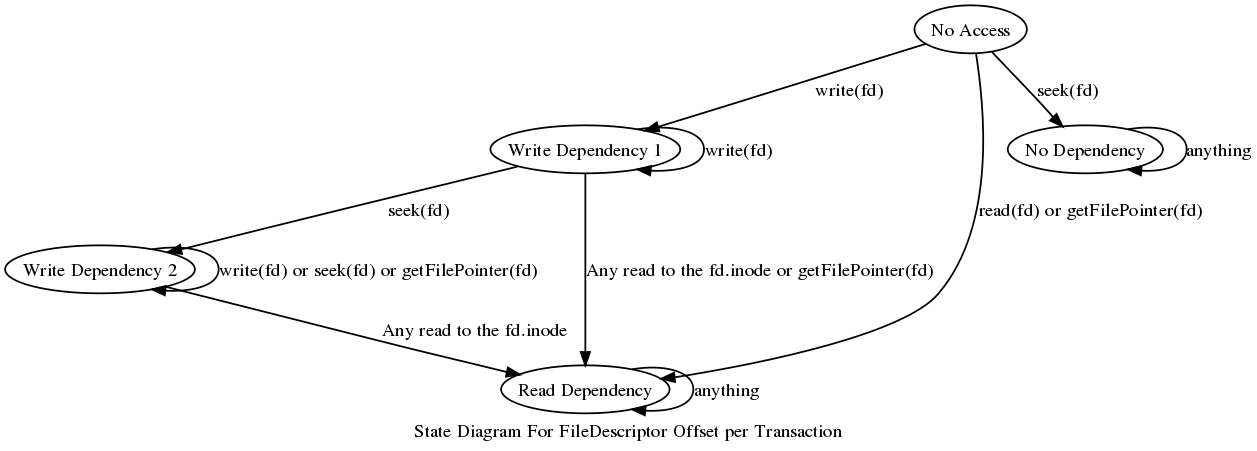
\includegraphics[scale = 0.3]{hello.png}\\

\textbf{Explanation}: Whenever the offset status for the transaction goes to "Read Dependence", a "forced-readoffset(fd)" operation is issued immediately preceding the operation that caused this transformation. The forced-radoofset(fd) is only issued if there is not a forced-readoffset(fd) in the $OP_{T_i}$ already.\\ 

\textbf{Axiom For Diagram:} If the first access to a filedescriptor is a $Seek(fd)$, then the following operation on $fd$ gets the offset value from the assignment made by the $Seek(fd)$ and advances the offset. Hence, the following operations get this offset and the offset value the filedescriptor had had before this transaction accesses fd is never referenced (thats why it is an absorbing state). This conforms to the definition of "None" state.\\ 

If $Read(fd.inode, offset, length)$ or $GetFilePointer(fd)$ is the first access made by this transaction, the offset is read (since the data needs to be read at this instant), this offset should be the one committed by a previously committed transaction (as this is the first access to $fd$ in this transaction). Once the offset is read, it is always dependent on this value (hence an absorbing state). For all the following operations, the offset value is known. This conforms to the definition that there is at least (the first read ever on fd by this transaction) one operation that acts on the offset value for fd and rules out the "Write Dependency" and "None" states.\\

If $Write(fd.inode, offset, length)$ is the first access made to fd by this transaction, then the offset to write to, can be decided at commit instant since the Write functions means start writing at the most recent committed fd.offset, hence offset realization can be postponed till commit instant. Any Writes or Seeks would still leave this dependency, since operations after a Seek act on absolute offset, and Writes preceding any Seek can all determine the offset at commit instant for the same reason as before.\\    

However, if a Read on the same fd in the transaction is invoked there are two possibilities:\\

1- A Seek precedes this Read, hence the offset value is absolute and is not read, however the ranges that are supposed to be written by Writes preceding the Seek, may overlap with the range Read is willing to Read from, and according to Rules(Most Recent Changes Should Be Visible) if thats the case the Read should be able to see this data, this suggests the ranges that all the Writes are going to write to should be realized now and this requires settling down on a value for all file descriptors offsets for this inode at this instant. Based on these, the most recent committed offset value for all these descriptors should be assigned to the offsets for the Writes that for the first time accessed the descriptor. Other for writes preceding the Seek, get this value as being advance by prior writes.\\

2- No Seek precedes the Read, hence the offset value the Read has to read from is unknown, since preceding Writes to fd have all used unknown offsets, the offset value given to Read is an unknown once, however it has to be known, follows that the offset value for the Write that for the first time accessed this fd should be decided upon and as shown before, the value should be the most recent committed offset value for fd. The offset value for this read or other writes, is the offset value obtained as being advanced by those operations.\\  

The two same possibilities exist when a GetFilePointer operation is invoked on the same fd:\\

1- If a Seek precedes it, then the offset value becomes absolute and hence the getFilePointer could retrieve the value assigned by Seek.\\

2- Otherwise, the offset value is still unknown, hence to be able to determine the offset value at this instant, the value obtained by reading the last committed offset value should be assigned to the offset value. for the first Write to $fd$.\\



%\textbf{Def 2-} \emph{Read and Write Operation}: 1- A Readdata is always a read operation. 2- ${readoffset(fd})\in OP_{T_i}$ is only a read operation, if it precedes a ${forceoffset(fd)} \in OP_{T_i}$. The reason is even though readoffset reads the offset, but the value does not matter unless specefied by ${forceoffset }$. 3- ${writeoffset}$ and ${writedata}$ are write operations.\\


%\textbf{Note 1-}: The runtime determines if and only if this is the first time the fd has been accessed by this transaction, then a $\{{offset} = {readoffset(fd)}\}$ is inserted in the sequence of operations. This ensures the offset is read for each filedescriptor once, and thats the first time it is accessed.\\

\subsection{User-Level Operations Structure}

The user-level operation cab be broken as follows:\\

1- Seek(fd): This operation sets the offset for filedescriptor. We define it as demonstarted below:\\

\hspace{8mm} Just an internal assignment in the transaction, $\{{fd.offset = value}\}$.\\  


2- Write(fd):\\

\hspace{8mm} 1- $\{writedata(fd.inode, offset, length), fd.offset = fd.offset + length\}$\\

3- GetFilePointer(fd):\\

\hspace{8mm} \{\{$forcedreadoffset(fd)$ issued as demonstrated at the state diagram if any, it is issued when the state for fd in this transaction is not in "No Dependency" or "Write Dependency 2"\}\}\\

4- Read(fd):\\

\hspace{8mm} $\forall filedescriptor fd_i$ where $fd_i.inode = fd.inode$ and the state for $fd_i$ in this transaction is not $No Dependency$, Read(fd) =$\{\{forcedreadoffset(fd_i)\}\}, {readdata(fd.inode, offset, length)}, offset = offset + length\}$\\

%\hspace{8mm}  1-  If ${read(fd)} \in OP_{T_i}$ and  $\exists forceoffset(fd) \in OP_{T_i}$ such that $forceoffset(fd) \rightarrow read(fd)$, then:\\

%\hspace{16mm} $\{{read(fd)}=readdata(fd.inode, offset, lenght), fd.offset = fd.offset + length\} $\\


%\hspace{8mm}  2-  If ${read(fd)} \in OP_{T_i}$ and  $ \not \exists forceoffset(fd) \in OP_{T_i}$ such that $forceoffset(fd) \rightarrow read(fd)$, then:\\

%\hspace{16mm} 1- If $\exists Seek(fd) \in USEROP_{T_i}$ such that $Seek(fd) \rightarrow read(fd)$ then:\\  

%\hspace{16mm} $\forall fd_i \in filedescriptors-accessed-by-T_i$ if $\exists writedata(fd_i.inode, offset, length)$ where $fd_i.inode = fd.inode$ and ${write(fd_i, offset, lenght)} \rightarrow {read(fd)}$  and $\not \exists seek(fd_i)$ such that $seek(fd_i) \rightarrow write(fd_i)$ and $\not \exists forceoffset(fd_i)$ such that $forceoffset(fd_i) \rightarrow read(fd)$ then ${read(fd)} = \{ \{forceoffset(fd_i)\},readdata(fd.inode, offset, length), fd.offset = fd.offset + length\}$ \\

%\hspace{16mm} 2- Else:\\ $\forall fd_i \in filedescriptors-accessed-by-T_i$ excluding $fd$ itself, if $ \exists writedata(fd_i.inode, offset, length)$ where ${write(fd_i, offset, lenght)} \rightarrow {read(fd)}$  and $\not \exists seek(fd_i)$ such that $seek(fd_i) \rightarrow write(fd_i)$ and $\not \exists forceoffset(fd_i)$ such that $forceoffset(fd_i) \rightarrow read(fd)$ then ${read(fd)} = \{ \{forceoffset(fd_i)\},readdata(fd.inode, offset, length), fd.offset = fd.offset + length\}$ \\

5- EndTransaction: 

\hspace{8mm} $\forall fd_i$ such that the state for $fd_i$ in this transaction is  not "No State",  $EndTransaction= \{\{{writeoffset(fd_i)}\}, commit\}$\\

Essentially for any fd that the correspondent state diagram in the transactions shows is in a state other than "No Access", a writeoffset(fd) is issued while committing.\\



\subsection{$writedata$ Dependecy on Offset}

Any writedata operation within a transaction gets $fd$ and an offset as arguments. There writes are reflected in the commit instant, however the offset to write to as we saw earlier for some writes i s determined at commit instant and for other is bound to a specific value before commit instant. We should have a policy to be able to diffrenciate between these two. The 3 rules below odes this.\\

1- If the state for $fd$ a given distinguish in a transaction is "Write Dependency 1" all writes by that transaction to that $fd$ will get the value of the offset to write to at commit instant (since in "Write Dependency 1" all writes are at unknown offsets) .\\\

2- If the state for $fd$ is "Read Dependency"  or "No Dependency" then all writes on $fd$ within this transaction should be done at offset determined for them when they were invoked (since all writes are to known offsets either determined by the transaction itself or a previously committed transaction).\\

3- Otherwise, if the state is "Write Dependency 2", then if the $writedata(fd.inode,...)$ operation precedes a $Seek(fd)$ then the offset is determined at commit instant (since all such writes are at unknown offset). Otherwise, the writes should be done at the offset decided upon earlier (the write after a Seek write the offset determined by Seek and hence to a known offset).\\


We could also think of this as a state machine for each writedata operation. The state diagram is created for each operation when it is first invoked and is subject to two things:\\

1- If there $\exists Seek(fd) or forced-readoffset(fd)\in OP_{T_i}$ such that those precede the $writedata(fd.inode,....)$ then the initial state in the state diagram for this writedata is Absolute.\\

2- Otherwise the initial state is Unknown offset.\\

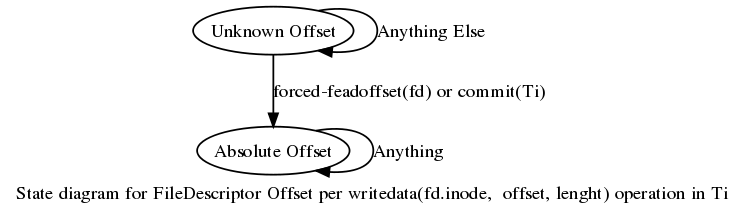
\includegraphics[scale = 0.3]{hello2.png}\\

The final state for all $writedata$ operations is Absolute, since the write should be perfomed at a specefic offset eventually. However, depending on the prevuious circumstances the system would immediately prior to commit determine the offset or would have realized it earlier.\\ 

\subsection{Guidelines for Implementaion}

As we saw earlier in Rule 4, any two operations can commute across each other unless they are subject to one of the two conditions in Rule 3.\\  

\textbf{Guideline 1}: \emph{Commuting forced-readoffset Operations}: A $forced-readoffset(fd) \in OP_{T_i}$ can go past a $commit_{T_j}$ if and only $\not \exists writeoffset(fd) in OP_{T_j}$.\\

\textbf{Axiom}: It follows immediately from Rule 4 and conditions in Rule 3, that this $forced-readoffset(fd)$ can go pats the commit. What remains to be proven is  $ \not \exists writeoffset(fd) \in OP_{T_i}$ such that it precedes 
$forced-readoffset(fd)$, as this would mean even if $\exists writeoffset \in OP_{T_j}$ still the $forced-readoffset(fd)$ could commute with $commit_{T_j}$.\\

This stems from the definition of EndTransaction operation, and the state diagram. A $forced-readoffset$ can be issued at any place in $OP_T{i}$ however it would always precede the $writeoffset(fd) \in OP_{T_i}$ since this is last operation in $OP_{T_i}$ before $commit$.\\

\textbf{Guideline 2}: \emph{Commuting readdata Operations}: A $readdata(fd_i.inode,offset_i, lenght_i) \in OP_{T_i}$ can go past a $commit_{T_j}$ if and only if \\

1- $\not \exists writedata(fd_j.inode, offset_j, length_j) in OP{T_j}$ such that $fd_j.inode= fd_i.inode$ and the two ranges $(offset_i, offset_i + length_i)$ and $(offset_i, offset_j + length_j)$ have an intersection.\\

 OR\\

2- $\exists$ a set of $writedata(fd_j.inode,offset_j, lenght_j) in OP_{T_i}$ such that for all of them $writedata \rightarrow readdata$ and $fd_i.inode = fd_j.inode$ and the range $(offset_i, offset_i + length)$ is a subrange for a combiantion of ranges for these $writedata$ operations.\\

\textbf{Axiom}: This follows imeediately from Rule 4 (1 and 2 are concrete representations for conditions 1 and 2 in Rule 3). However, it should be noted that whenever a $readata$ operation wants to commute across a $commit$ operation $\in T_j$, if $ \exists writedata \in OP_{T_j}$, the offset for the $wtitedata$ operation is known at this instant (according to the state diagram demonstarted below and regardless of whether $i = j$ or not), hence it would be trivial to see whether these $writedata$ operations intersect (or include in case they are in the same transaction as the $readata$) with the $readdata$ or not.\\

\textbf{Guideline 3:} \emph{Reads Should be Validated At Commit Instant}:
If an operation $a$ that "reads" some data $r_n$ (reads the data at some $t < t_{commit-of-the-transaction}$(the commit instant)), it should be ensured that the data $r_n$ is still valid in the actual file system at $t_{commit-of-the-transaction}$ (commit instant) or $T_i$ has to abort.\\

\textbf{Axiom}: If the data is not valid anymore it means the data $r_n$ has been written since $t_{i-1}$. This implies at least one operation $b$ has written the data since the use and $b$ does not precede $a$ and $a$ precedes $b$. $b$ is either an operation in the same transaction or a different one. However, if $b$ is in the same transaction, then the data read is valid at commit instant by defenition. On the other hand, assume $b$ belongs to a different transaction namely $T_j$. Since $T_j$ should have already commited, according to Corrolary 2 all operation in $OP_{T_j}$ should precede those in $OP_{T_i}$, however, we know there is at least an operation $b$ that does not precede $a$ (since $a$ has not seen the "writes" made to $r_n$ by $b$). Hence, $T_i$ can not commit.\\


\textbf{Guideline 4}: \emph{If Reads Are Valid At Commit Instant, the Transaction Commits}: If by applying Guideline 3 for $T_i$ it is ensured that $\forall r_i \in R{T_i}$ (all data read by $T_i$) is still valid at commit instant, then $\forall T_j \in T_{committed} T_j \rightarrow T_j$ and hence according to Rule 4 $T_i$ commits.\\

\textbf{Axiom}: If all data read is still valid at commit instant, means all operation in the set of operations belonging to committed transactions, can be relocated to precede those in $T_i$ (since no writes have been seen), and consequently all those transactions precede $T_i$. Rule 5 ensures such transaction would be able to commit.\\ 

\textbf{Guideline 5}: \emph{A Transaction About to Commit Can Abort Other Transaction Safely}: A transaction about to commit can check to what resources it has alreay written (denote this as $R_i$), an then $\forall T_j in T$  such that $T_j$ is active at this instant can check to see if any of those have read $r_i \in R_i$, if so and no other operation in $OP_{T_j}$ preceding this read has written to $r_i$ then $T_i$ can abort $T_j$, since $T_j$ is doomed to abrot anyway (according to Guideline 3).\\ 
 

\section{System Implementation Overview}

\subsection{Components}

In this sextion we will show how our system conforms to the guidlines and rules required by the system. Only the main components of the system are depicted in the figure and listed below. It should be noted that even for theses classes the major functions and fields are exposed in the illustration.\\

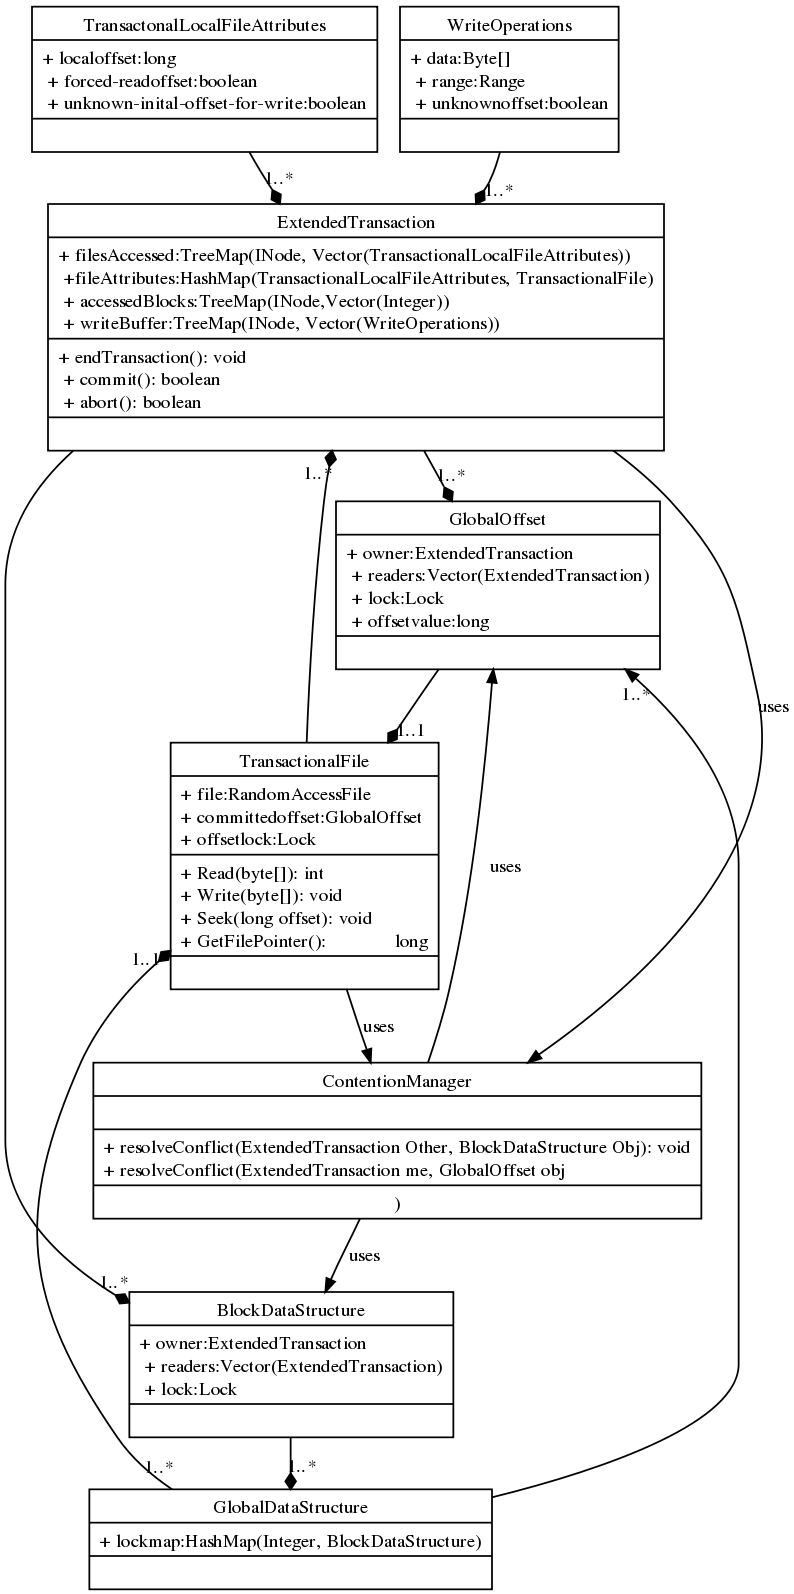
\includegraphics[scale = 0.3]{uml.png}\\

\textbf{TransactionalFile}: This is the object most user-level operations are perfomed on. It can be either created inside or outside a transaction. Accessing a TransactionalFile by $T_i$ means $T_i$ has invoked a user-level operation on the object. A Transactionalfile can be shared among any subset of the members of $T$. If shared, the offset is shared between these as well.\\

\textbf{ExtendedTransaction}: The class and data structures required to do the actions required by a transaction (commit, abort, ...).\\

\textbf{TransactionalLocalFileAttributes}: The class to maintain the data structures specific to a transaction regarding an already accessed TransactionalFile object (offset status for the transaction, inital offset status for each Write operation and etc.).\\

\textbf{GlobalOffset}: The class to maintain the global offset assosiated with each TransactionalFile object (the value, who owns the offset, who reads the offset, etc.) \\

\textbf{GlobalDataStructure}: The class to maintain the global data structure assosiated with each inode (such as mapping of block locks for each inode).\\

\textbf{ConflictManager}: The manager to resolve the conflict, this can be  when a transaction can not successfully commit  or a read or write has to do subsidary actions regarding other transaction or conflict over locks and etc.\\ 

\textbf{BlockDataStructure}: The data structure representing a block in an inode. GlobalDataStructure uses instances of this class to preserve the info
rmation.\\

\textbf{WriteOperation}: The structure of a writedata operatin, including the range it is supposed to write, the data to be written and wether this is an absolute or unknown offset value.\\

\subsection{Algorithm}

In this section we examine the psudecode for user-level operations in the propsed system and show how our system conforms to the formalisatiom buitl up in earlier sections.

\textbf{$tf_i$.Read(data[])}{\\

\hspace{8mm} If (tfla = currenttransaction.accessedfile.contains($tf_i$))

\hspace{11mm}	for any of the writes in writeuffer to $tf_i$.inode

\hspace{14mm}		if [tfla.localoffset, tfla.offset + data.length] overlaps with range for the write

\hspace{17mm}			copy the intersect portion to the correspondent portion of data[]

\hspace{11mm}	if any non-filled portion of data[] exists{

\hspace{14mm}		try to lock $tf_i$.offset.lock
	
\hspace{14mm}		try to lock all the blocks within range [tfla.localoffset, tfla.offset + data.length]

\hspace{14mm}		if all locks succeed then read the non-filled portions from $tf_i$.file

\hspace{14mm}		if not succeed consult contentionManager to resolve the conflict

\hspace{8mm} else add $tf_i$.inode to files accessed by this transaction and create the corresponding TransactionalLocalFileAttributes and call Read(data[])



\end{document}
